\documentclass{dlmubachelor}

\dlmubachelorset{%
	title=大连海事大学本科毕业设计(论文)\\ \LaTeX 文档类, % 论文中文标题,太长可用\\折行
	institute=船舶与海洋工程学院, % 学院
	majorclass=能源与动力工程3班, % 专业班级
	name=姓名,  % 姓名
	mentor=指导教师,    % 指导教师
	date=二〇二一年六月   % 完成日期
}

%% 页面设置,如果打印装订线(将left设置为3cm)取消下面的注释即可,建议提交老师的文档不打印装订线(left默认为2.5cm),打印纸质版文档打印装订边
%\geometry{left=3cm}

%% 这个命令用于在正文页眉打印标题,不用折行
\renewcommand{\onelinetitle}{大连海事大学本科毕业设计(论文)\LaTeX 文档类}

\begin{document}
%% cls文类中设置出了一些bug,导致正文字体变为了五号字体,没查到bug的位置,只好在此设置正文字体的字号了
\zihao{-4}
\maketitle

%% 摘要页及目录页眉页脚设置
\setcounter{page}{1}
\pagenumbering{Roman} % 设置页码格式为大写罗马字母
\pagestyle{plain}

%% include命令中tex的文件名不要写扩展名,否则不能编译出文件内容(不会报错),千万不要带扩展名!!!而且,不要include父文件夹的文件,否则编译报错误!!!
% 中文摘要
\begin{cnabstract}
	dlmubachelor.cls:一个适用于大连海事大学理工类本科生毕业论文的\LaTeX 文类;

	根据大连海事大学毕业设计(论文)工作手册(2011年11月版)的要求制作而成;

	基本满足大连海事大学毕业设计(论文)工作手册的要求。

	本文是dlmubachelor.cls使用的一个案例,希望能帮助大家!
	% 中文关键词
	\keywordscn 大连海事大学;本科毕业论文;\LaTeX 文类
\end{cnabstract}

% 英文摘要
\begin{enabstract}
	dlmubachelor.cls is a \LaTeX\ documentclass suitable for Dalian Maritime University bachelor's degree thesis;

	It is based on the requirements of the graduation design (thesis) manual of Dalian Maritime University ( November 2011 edition ) and it generally meets the requirements of the graduation design (thesis) manual of Dalian Maritime University.

	This article is a simple example of dlmubachelor.cls, hoping it can help you!
	% 英文关键词
	\keywordsen Dalian Maritime University; Bachelor's degree thesis; \LaTeX\ documentclass
\end{enabstract}
 % 摘要页
\phantomsection\addcontentsline{toc}{section}{目\hspace{2em}录}
\tableofcontents
\newpage

%% 正文页眉页脚设置
\setcounter{page}{1}
\fancypagestyle{plain}{
	\fancyhf{} % 清空页眉页脚
	\chead{\zihao{5}\onelinetitle}
	\cfoot{\zihao{5}\thepage}
	\renewcommand{\headrulewidth}{0.4pt}
}
\pagestyle{plain} % 使用重新定义的plain格式
\pagenumbering{arabic} % 设置页码格式为阿拉伯数字


%% 正文

\centerline{\bf\zihao{3}\onelinetitle}
\section{文类简介、选项与设置}
\subsection{文类简介}
\textbf{本文类是在TeX Live 2021环境下编写的,需要采用xelatex进行编译,虽然是TeX Live 2021版本,但老版本的TeX Live也应该能编译成功。}本文类可能不支持老旧的CTeX套装,但也欢迎大家使用CTeX环境尝试,如果能编译成功欢迎大家使用!CTeX套装因为WinEdt的版权问题早已无人维护,中文的LaTeX排版采用成熟的ctex宏包更为方便。文类已经加载的宏包有:ctex, geometry, fontenc, mathptmx, xkeyval, titlesec, titletoc, amsmath, amsfonts, amssymb, bm, array, longtable, booktabs, multirow, graphicx, subfig, flafter, caption, hyperref, cleverref, ulem, xcolor, fancyhdr, listings, paralist。
\subsection{选项与设置}
本文类提供了title、institute、majorclass、name、mentor、date等宏包选项,对应的分别是论文题目、所在学院、专业班级、姓名、指导教师、日期等项目。若论文题目太长,可用\textbackslash\textbackslash 使其折行,例如本文的相关的设置为

\centerline{title = 大连海事大学本科毕业设计(论文)\textbackslash\textbackslash\ \textbackslash LaTeX 文档类}

另外,定义了一个onelinetitle的命令,用于在页眉输出一行形式的题目,在重新定义onelinetitle处,只需把title中的\textbackslash\textbackslash 删除然后赋给onelinetitle即可。其他设置比较简单,可见template-example.tex文件的相关设置。

欢迎大家去海大\LaTeX\ 学习交流群讨论相关技术问题,\textbf{QQ群号码为:835453813}
\subsubsection{三级标题}
这里是三级标题的测试。
\paragraph{四级标题}
这里是四级标题的测试,但四级标题并不会出现在目录。
 % 第一章
\centerline{\bf\zihao{3}\onelinetitle}
\section{文类简介、选项与设置}
\subsection{文类简介}
\textbf{本文类是在TeX Live 2021环境下编写的,需要采用xelatex进行编译,虽然是TeX Live 2021版本,但老版本的TeX Live也应该能编译成功。}本文类可能不支持老旧的CTeX套装,但也欢迎大家使用CTeX环境尝试,如果能编译成功欢迎大家使用!CTeX套装因为WinEdt的版权问题早已无人维护,中文的LaTeX排版采用成熟的ctex宏包更为方便。文类已经加载的宏包有:ctex, geometry, fontenc, mathptmx, xkeyval, titlesec, titletoc, amsmath, amsfonts, amssymb, bm, array, longtable, booktabs, multirow, graphicx, subfig, flafter, caption, hyperref, cleverref, ulem, xcolor, fancyhdr, listings, paralist。
\subsection{选项与设置}
本文类提供了title、institute、majorclass、name、mentor、date等宏包选项,对应的分别是论文题目、所在学院、专业班级、姓名、指导教师、日期等项目。若论文题目太长,可用\textbackslash\textbackslash 使其折行,例如本文的相关的设置为

\centerline{title = 大连海事大学本科毕业设计(论文)\textbackslash\textbackslash\ \textbackslash LaTeX 文档类}

另外,定义了一个onelinetitle的命令,用于在页眉输出一行形式的题目,在重新定义onelinetitle处,只需把title中的\textbackslash\textbackslash 删除然后赋给onelinetitle即可。其他设置比较简单,可见template-example.tex文件的相关设置。

欢迎大家去海大\LaTeX\ 学习交流群讨论相关技术问题,\textbf{QQ群号码为:835453813}
\subsubsection{三级标题}
这里是三级标题的测试。
\paragraph{四级标题}
这里是四级标题的测试,但四级标题并不会出现在目录。
 % 第一章

\section{公式、表格与插图}
文类使用了cleverref宏包,这使得公式、表格与插图的交叉引用非常智能化。
\subsection{公式}
公式的一个简单例子:

\cref{gougueq}是勾股定理的公式,其中$ a\text{、}b $表示两个直角边,$ c $表示斜边。
\begin{equation}
	\label{gougueq}
	a^2+b^2=c^2
\end{equation}

其代码如下:
\begin{verbatim}
	\cref{gougueq}是勾股定理的公式,其中$ a\text{、}b $表示两个直角边,$ c $表示斜边。
	\begin{equation}
		\label{gougueq}
		a^2+b^2=c^2
	\end{equation}
\end{verbatim}
\subsection{表格}
这里主要演示三线表的使用,\cref{tab1}展示了文类使用的一些宏包。
\begin{table}[htbp]
	\centering
	\caption{文类使用的部分宏包}
	\label{tab1}
	\begin{tabular}{cc}
		\toprule[1pt]
		% 我比较喜欢这样改宽度
		\hspace{1cm}宏包\hspace{1cm} & \hspace{3cm}作用\hspace{3cm} \\
		\midrule[0.5pt]
		ctex                         & 支持排版中文                 \\
		geometry                     & 调整页面布局                 \\
		titlesec                     & 标题格式设置                 \\
		titletoc                     & 目录格式设置                 \\
		amsmath                      & 多种公式环境                 \\
		amsfonts                     & 数学符号、字体               \\
		amsmb                        & 数学符号、字体               \\
		bm                           & 数学粗体                     \\
		\bottomrule[1pt]
	\end{tabular}
\end{table}

下面是有关的代码,\textbf{需要强调的是:}{\color[rgb]{1.00,0.00,0.00}一定要让label写在caption后,否则交叉引用会不正确!!!}
\begin{verbatim}
	\begin{table}[htbp]
		\centering
		\caption{文类使用的部分宏包}
		\label{tab1}
	\begin{tabular}{cc}
	\toprule[1pt]
	% 我比较喜欢这样改宽度
	\hspace{1cm}宏包\hspace{1cm}	&	\hspace{3cm}作用\hspace{3cm}	\\
			\midrule[0.5pt]
			ctex	& 	支持排版中文	\\
			geometry	&	调整页面布局	\\
			titlesec	&	标题格式设置	\\
			titletoc	&	目录格式设置	\\
			amsmath	&	多种公式环境	\\
			amsfonts	&	数学符号、字体	\\
			amsmb	&	数学符号、字体	\\
			bm	&	数学粗体	\\
			\bottomrule[1pt]
		\end{tabular}	
	\end{table}
\end{verbatim}

\subsection{图片}
文类使用了graphicx,subfig宏包来排版图片,\cref{ctanlion}是单图排版的一个简单例子。
\begin{figure}[htbp]
	\centering
	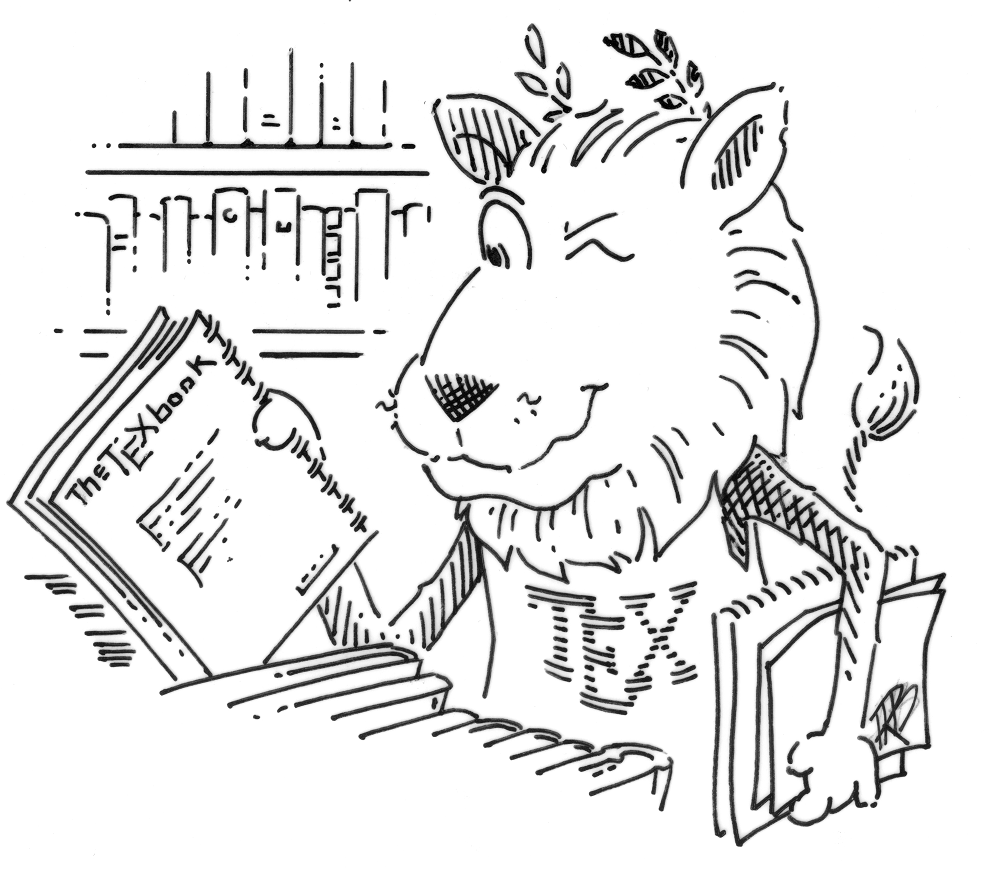
\includegraphics[width=0.6\linewidth]{ctan_lion}
	\caption{ctan小狮子}
	\label{ctanlion}
\end{figure}

其代码如下:
\begin{verbatim}
	\begin{figure}[htbp]
		\centering
		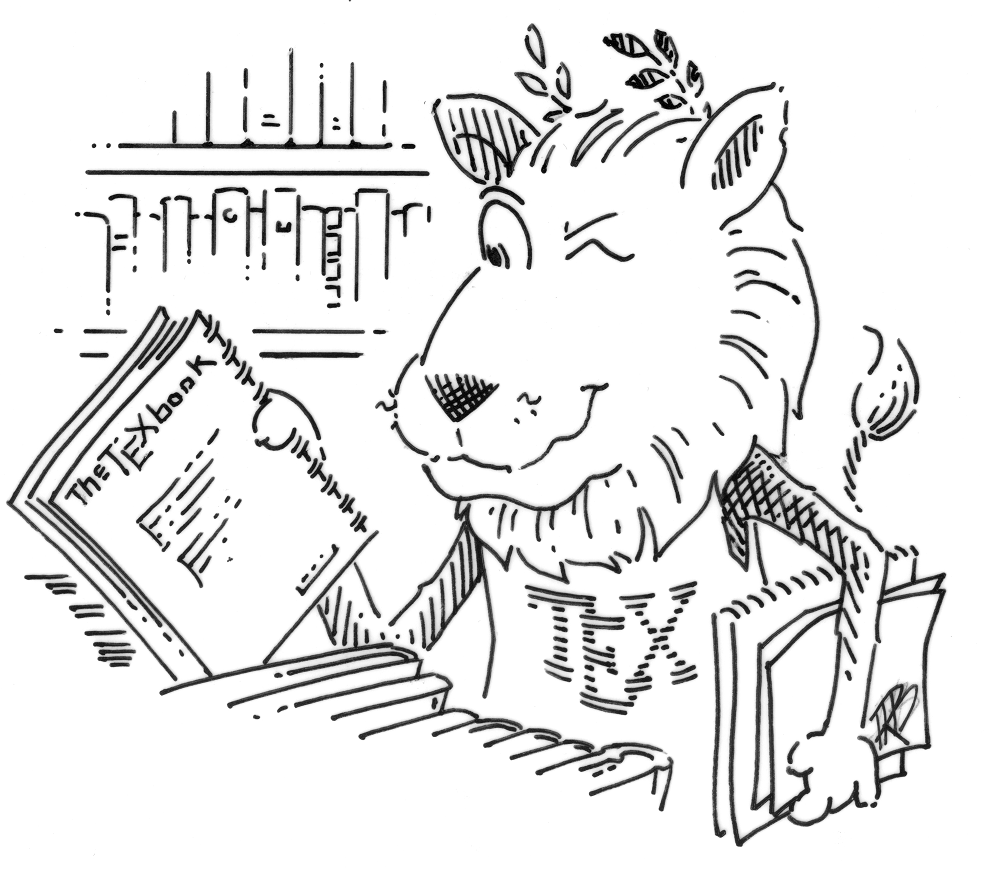
\includegraphics[width=0.6\linewidth]{ctan_lion}
		\caption{ctan小狮子}
		\label{ctanlion}
	\end{figure}
\end{verbatim}

\cref{twofig}是双图排版的一个简单案例,其中\cref{sf:ctanlion}是ctan官网小狮子,\cref{sf:colorful}是着色的小狮子。

\begin{figure}[htbp]
	\centering
	\subfloat[ctan小狮子\label{sf:ctanlion}]{
		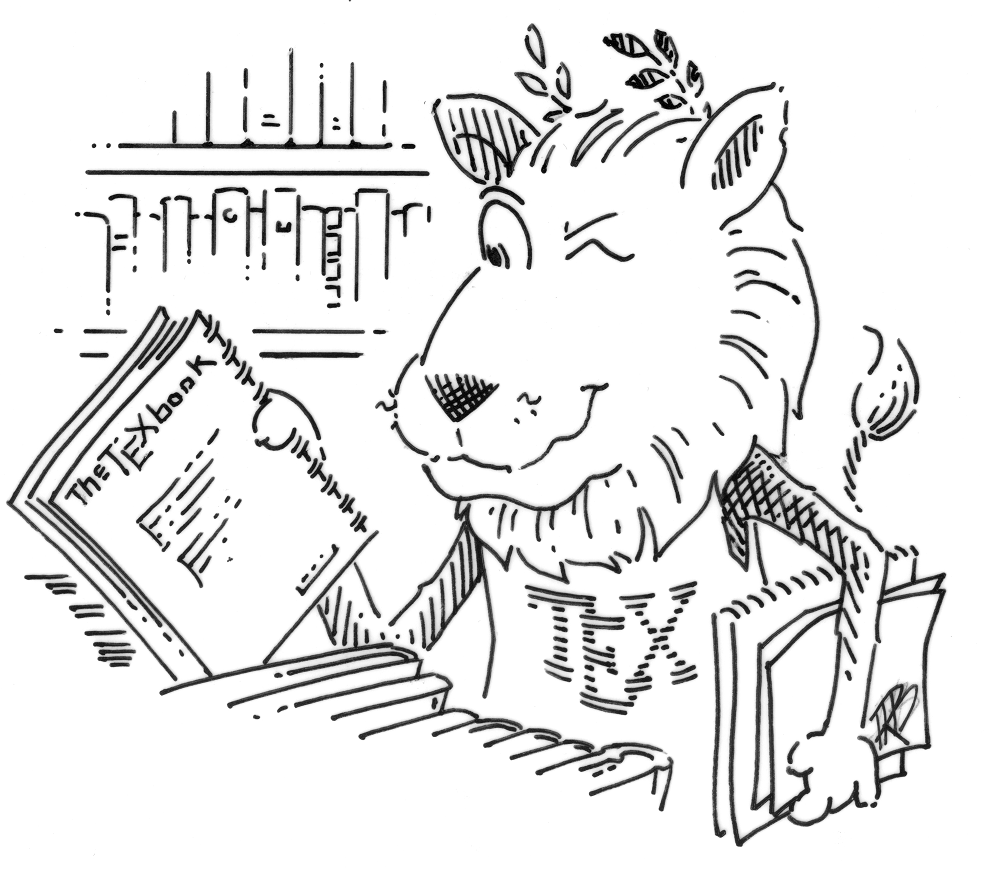
\includegraphics[width=0.3\linewidth]{ctan_lion}
	}
	\hspace{1em}
	\subfloat[着色小狮子\label{sf:colorful}]{
		
\includegraphics[width=0.3\linewidth]{colorful_lion}
	}
	\caption{双图排版}
	\label{twofig}
\end{figure}

下面是相相关代码:
\begin{verbatim}
	\begin{figure}[htbp]
		\centering
		\subfloat[ctan小狮子\label{sf:ctanlion}]{
			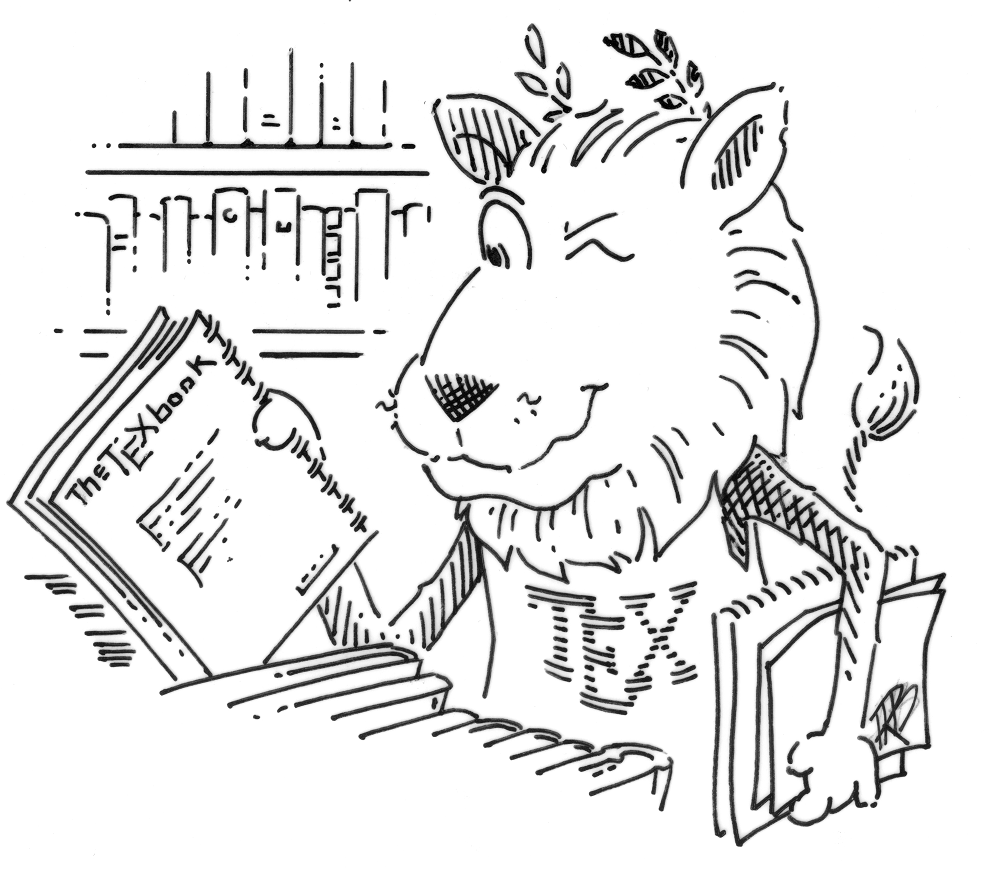
\includegraphics[width=0.3\linewidth]{ctan_lion}
		}
		\hspace{1em}
		\subfloat[着色小狮子\label{sf:colorful}]{
			
\includegraphics[width=0.3\linewidth]{colorful_lion}
		}
		\caption{双图排版}
		\label{twofig}
	\end{figure}
\end{verbatim}

\cref{twofig2}是另一种双图排版的实现方法,\textbackslash subfloat命令缺少宽度参数,而子标题最多只能和子图一样宽,太长的话会出现折行。为了避免子标题折行,\textbackslash subfloat里再嵌套个minipage,因为后者是有宽度的\upcite{btl}。在此处页展示了参考文献上标引用方法,其命令为\verb|\upcite{btl}|;若不需要上标形式,即\cite{btl}这种格式,可直接用cite引用命令。\textbf{需要注意的是,图片的宽度要小于minipage环境的宽度才能正确排版出图片!!!}

\begin{figure}[htbp]
	\centering
	\subfloat[ctan小狮子\label{sf:ctanlion2}]{
		\begin{minipage}{5cm}
			\centering
			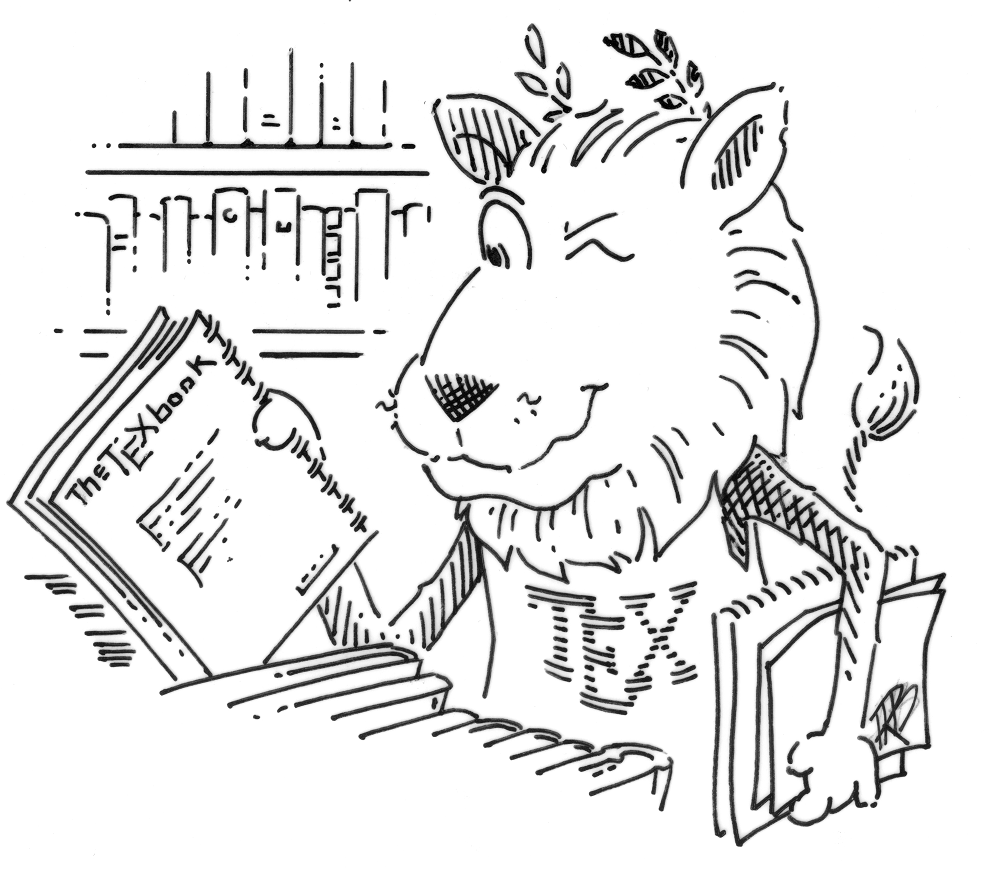
\includegraphics[width=4.5cm]{ctan_lion}
		\end{minipage}
	}
	\subfloat[着色小狮子\label{sf:colorful2}]{
		\begin{minipage}{5cm}
			\centering
			
\includegraphics[width=4.5cm]{colorful_lion}
		\end{minipage}
	}
	\caption{另一种双图排版}\label{twofig2}
\end{figure}


下面是相关代码:
\begin{verbatim}
	\begin{figure}[htbp]
		\centering
		\subfloat[ctan小狮子\label{sf:ctanlion2}]{
			\begin{minipage}{5cm}
				\centering
				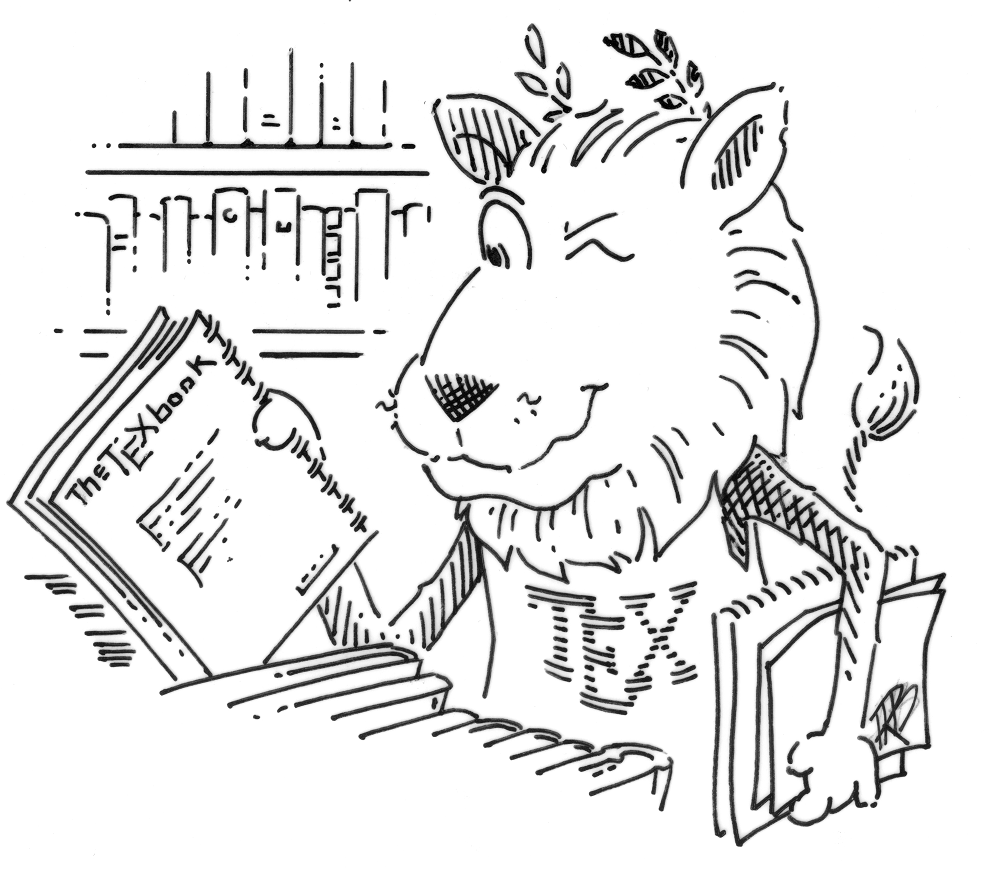
\includegraphics[width=4.5cm]{ctan_lion}
			\end{minipage}
		}
		\subfloat[着色小狮子\label{sf:colorful2}]{
			\begin{minipage}{5cm}
				\centering
				
\includegraphics[width=4.5cm]{colorful_lion}
			\end{minipage}
		}
		\caption{另一种双图排版}\label{twofig2}
	\end{figure}
\end{verbatim}

 % 第二章

\newpage
\section*{结论}
\phantomsection\addcontentsline{toc}{section}{结论}
%% 上面东西不要动,在下面直接写结论!!!
上面东西不要动,删除此行后直接在此处写结论!!!上面东西不要动,删除此行后直接在此处写结论!!!上面东西不要动,删除此行后直接在此处写结论!!!上面东西不要动,删除此行后直接在此处写结论!!!上面东西不要动,删除此行后直接在此处写结论!!!上面东西不要动,删除此行后直接在此处写结论!!!上面东西不要动,删除此行后直接在此处写结论!!!上面东西不要动,删除此行后直接在此处写结论!!!上面东西不要动,删除此行后直接在此处写结论!!!



\newpage % 结论

\begin{thebibliography}{99}
	\phantomsection\addcontentsline{toc}{section}{参\hspace{1ex}考\hspace{1ex}文\hspace{1ex}献}\zihao{5} % 此行不可改动,从下面插入bibitem条目
	\bibitem{lhy} 刘海洋. \LaTeX 入门[M]. 电子工业出版社, 2013.
	\bibitem{hw} 胡伟. \LaTeXe 完全学习手册(第2版)[M]. 清华大学出版社, 2013.
	\bibitem{btl} 包太雷. \LaTeX\ NOTES —— 雷太赫排版系统简介(第二版)[M/OL]. 2019.\url{http://static.latexstudio.net/article/2019/0504/lnotes-master.zip}
\end{thebibliography}
\newpage % 参考文献

\begin{thinking}
	衷心感谢哈工大博士生乙醇学长(笔名)给我技术上的指导和帮助,乙醇学长的回答既给了我准确的帮助,又让我了解到一些查阅问题帮助的途径,再次表示对您的感谢!
	
	感谢能源与动力工程系李博健同学对模板编写工作的关心和支持,目前李博健同学已经使用本模板完成了专题部分的论文,写作过程中发现了一些重要问题,目前已经修改完毕!
\end{thinking} % 致谢

\setcounter{page}{1}
\fancypagestyle{plain}{
	\fancyhf{} % 清空页眉页脚
	\chead{}
	\cfoot{\zihao{5}\thepage}
	\renewcommand{\headrulewidth}{0pt}
}
\pagestyle{plain}
\zihao{5}
\newpage
\phantomsection\addcontentsline{toc}{section}{附录1}
{\noindent\zihao{4}\bf\vspace{0.5\baselineskip}附录1\vspace{0.5\baselineskip}}\par
若无附录2,可将下面内容注释掉。


\newpage
\phantomsection\addcontentsline{toc}{section}{附录2}
{\noindent\zihao{4}\bf\vspace{0.5\baselineskip}附录2\vspace{0.5\baselineskip}}\par
若还需附录3等,可类似复制上面内容并更改掉相应的数字!!! % 附录


\end{document}